
\documentclass[a4paper,12pt]{article}
%%%%%%%%%%%%%%%%%%%%%%%%%%%%%%%%%%%%%%%%%%%%%%%%%%%%%%%%%%%%%%%%%%%%%%%%%%%%%%%%%%%%%%%%%%%%%%%%%%%%%%%%%%%%%%%%%%%%%%%%%%%%%%%%%%%%%%%%%%%%%%%%%%%%%%%%%%%%%%%%%%%%%%%%%%%%%%%%%%%%%%%%%%%%%%%%%%%%%%%%%%%%%%%%%%%%%%%%%%%%%%%%%%%%%%%%%%%%%%%%%%%%%%%%%%%%
\usepackage{eurosym}
\usepackage{vmargin}
\usepackage{amsmath}
\usepackage{graphics}
\usepackage{epsfig}
\usepackage{subfigure}
\usepackage{fancyhdr}

\setcounter{MaxMatrixCols}{10}
%TCIDATA{OutputFilter=LATEX.DLL}
%TCIDATA{Version=5.00.0.2570}
%TCIDATA{<META NAME="SaveForMode"CONTENT="1">}
%TCIDATA{LastRevised=Wednesday, February 23, 201113:24:34}
%TCIDATA{<META NAME="GraphicsSave" CONTENT="32">}
%TCIDATA{Language=American English}

\pagestyle{fancy}
\setmarginsrb{20mm}{0mm}{20mm}{25mm}{12mm}{11mm}{0mm}{11mm}
\lhead{MA4128} \rhead{Kevin O'Brien} \chead{Assumptions for Linear Models} %\input{tcilatex}

\begin{document}
	
	\tableofcontents
	\newpage
	
	
	
	
\section{Linear Regression Analysis}

\subsection{Introduction}
\begin{itemize}
\item Linear regression is used when you want to predict the value of a variable based on the value of another variable. The variable we want to predict is called the dependent variable (or sometimes, the outcome variable). The variable we are using to predict the other variable's value is called the independent variable (or sometimes, the predictor variable).


\item For example, you could use linear regression to understand whether exam performance can be predicted based on revision time; whether cigarette consumptions can be predicted based on smoking duration; and so forth. If you have two or more independent variables, rather than just one, you need to use \textbf{\textit{multiple regression}}.

\item SPSS can be used to carry out linear regression, as well as interpret and report the results from this test. However, before we introduce you to this procedure, you need to understand the different assumptions that your data must meet in order for linear regression to give you a valid result. We discuss these assumptions next.

\end{itemize}


\subsection{Importance of Testing Model Assumptions}
\begin{itemize}
\item When you choose to analyse your data using linear regression, part of the process involves checking to make sure that the data you want to analyse can actually be analysed using linear regression. You need to do this because it is only appropriate to use linear regression if your data is appropriate for six assumptions that are required for linear regression to give you a valid result.

\item In practice, checking for these six assumptions just adds a little bit more time to your analysis, requiring you to click a few more buttons in SPSS when performing your analysis, as well as think a little bit more about your data, but it is not a difficult task.

\item Often when analysing your own data using SPSS, one or more of these assumptions is violated (i.e., not met). This is not uncommon when working with real-world data rather than textbook examples, which often only show you how to carry out linear regression when everything goes well. However, even when your data fails certain assumptions, there is often a solution to overcome this. 
\end{itemize}

\subsection*{Assumptions}
First, let’s take a look at these six assumptions:
\begin{itemize}
\item \textbf{Assumption 1}: Your two variables should be measured at the interval or ratio level (i.e., they are continuous). Examples of variables that meet this criterion include revision time (measured in hours), intelligence (measured using IQ score), exam performance (measured from 0 to 100), weight (measured in kg), and so forth.
% You can learn more about interval and ratio variables in our article: Types of Variable.

\item \textbf{Assumption 2}: There needs to be a linear relationship between the two variables. Whilst there are a number of ways to check whether a linear relationship exists between your two variables, we suggest creating a scatter-plot using SPSS, where you can plot the dependent variable against your independent variable, and then visually inspect the scatter-plot to check for linearity. Your scatter-plot may look something like one of the following:

If the relationship displayed in your scatterplot is not linear, you will have to either run a non-linear regression analysis or \textbf{\textit{transform}} your data, which you can do using SPSS. It is important to learn how to: \begin{itemize}
\item[(a)] create a scatterplot to check for linearity when carrying out linear regression using SPSS; \item[(b)] interpret different scatterplot results \item[(c)] transform your data using SPSS if there is not a linear relationship between your two variables.
\end{itemize}

\begin{figure}[h!]
\begin{centering}
  % Requires \usepackage{graphicx}
  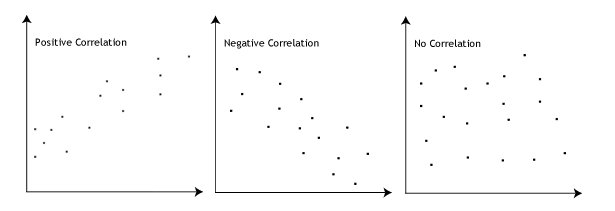
\includegraphics[width=10cm]{images/Regre1.jpg}\\
  \caption{Types of Linear Relationship}
\end{centering}
\end{figure}

\item \textbf{Assumption 3}: There should be no significant outliers. Outliers are simply single data points within your data that do not follow the usual pattern (e.g., in a study of 100 students’ IQ scores, where the mean score was 108 with only a small variation between students, one student had a score of 156, which is very unusual, and may even put her in the top 1\% of IQ scores globally). The following scatterplots highlight the potential impact of outliers:

The problem with outliers is that they can have a negative effect on the regression equation that is used to predict the value of the dependent (outcome) variable based on the independent (predictor) variable. This will change the output that SPSS produces and reduce the predictive accuracy of your results. Fortunately, when using SPSS to run linear regression on your data, you can easily include criteria to help you detect possible outliers.
\begin{figure}[h!]
\begin{centering}
  % Requires \usepackage{graphicx}
  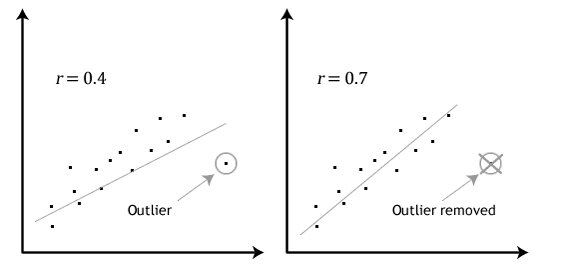
\includegraphics[width=10cm]{images/Regre2.jpg}\\
  \caption{Effect of an Outlier}
\end{centering}
\end{figure}
%In our enhanced linear regression guide, we: (a) show you how to detect outliers using \textbf{case-wise diagnostics}, which is a simple process when using SPSS; and (b) discuss some of the options you have in order to deal with outliers.
\item \textbf{Assumption 4}: You should have independence of observations, which you can easily check using the Durbin-Watson statistic, which is a simple test to run using SPSS. We explain how to interpret the result of the Durbin-Watson statistic later.

\item \textbf{Assumption 5}:Your data needs to show \textbf{\textit{homoscedasticity}}, which is where the variances along the line of best fit remain similar as you move along the line. Whilst we explain more about what this means and how to assess the homoscedasticity of your data in the linear regression line, take a look at the two scatter-plots below, which provide two simple examples: one of data that meets this assumption and one that fails the assumption:

\begin{figure}[h!]
\begin{centering}
  % Requires \usepackage{graphicx}
  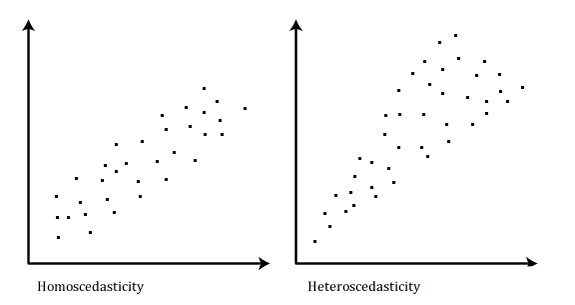
\includegraphics[width=10cm]{images/Regre3.jpg}\\
  \caption{Constant Variance}
\end{centering}
\end{figure}
When you analyse your own data, you will be lucky if your scatterplot looks like either of the two above. Whilst these help to illustrate the differences in data that meets or violates the assumption of homoscedasticity, real-world data is often a lot more messy. Therefore, in our enhanced linear regression guide, we explain: (a) some of the things you will need to consider when interpreting your data; and (b) possible ways to continue with your analysis if your data fails to meet this assumption.
\item \textbf{Assumption 6}:Finally, you need to check that the residuals (errors) of your two variables are approximately normally distributed (we explain these terms in our enhanced linear regression guide). Two common methods to check this assumption include using either a histogram (with a superimposed normal curve) or by using a Normal P-P Plot.
  %  Again, in our enhanced linear regression guide, we: (a) show you how to check this assumption using SPSS, whether you use a histogram (with superimposed normal curve) or Normal P-P Plot; (b) explain how to interpret these diagrams; and (c) provide a possible solution if your data fails to meet this assumption.

\end{itemize}
You can check assumptions all assumptions except no.1 using SPSS. It is recommended to test these assumptions in this order because it represents an order where, if a violation to the assumption is not correctable, you will no longer be able to use a single linear regression (although you may be able to run another statistical test on your data instead). Just remember that if you do not run the statistical tests on these assumptions correctly, the results you get when running a linear regression might not be valid.


\end{document}
%------------------------------------------------------------------------------%\end{document}


